\documentclass{ximera}

\author{Anna Davis} \title{MTH 140 Homework 5} 

\begin{document}

\begin{abstract}

\end{abstract}
\maketitle
 \textit{Certificate due: 10/5/2020 at 11:59 p.m.}
\begin{problem}\label{prob:140hom5prob1}
Normal distribution.
\begin{enumerate} 
\item
Approximately what percent of values from a normal distribution lie within one standard deviation of the mean? (State your answer to the nearest integer.)
$$\answer{68}\%$$
\item Approximately what percent of values from a normal distribution lie OUTSIDE of two standard deviations from the mean?  (State your answer to the nearest integer.)
$$\answer{5}\%$$
\item Suppose $X\sim N(25, 4)$.  Then approximately 68\% of the points lie between \wordChoice{\choice{19 and 31}, \choice[correct]{21 and 29},\choice{23 and 27}}

\item All of the questions above illustrate the use of \wordChoice{\choice[correct]{the Empirical Rule}, \choice{Central Limit Theorem},\choice{Continuous Distribution Law},\choice{Normal Distribution Law}}
\end{enumerate}

\end{problem}

\begin{problem}\label{prob:140hom5prob2}
Suppose the amount of sugar in a cookie is normally distributed with $\mu=31.4$ grams and $\sigma=1.1$ grams.  Use GeoGebra to answer the questions.  Geogebra gives answers to four decimal places.  State your answers using all of the digits from GeoGebra.
\begin{center}  
\geogebra{emwxhga2}{800}{600}  
\end{center}
\begin{enumerate}
    \item What percentage of cookies will contain less than 30 grams of sugar?
    $$\answer{10.16}\%$$
    \item What is the probability of a randomly selected cookie containing 32 or more grams of sugar?
    $$\answer{0.2927}\mbox{ not percent; just decimal}$$
    \item What percentage of cookies will contain between 32 and 33 grams of sugar?
    $$\answer{21.98}\%$$
    \item Find the z-score for a cookie containing 34 grams of sugar.  (Round to two decimal places.)
    $$z=\answer{2.36}$$
\end{enumerate}
\end{problem}

\begin{problem}\label{prob:140hom5prob5}
Depicted below is the distribution $X\sim N(13, \sigma)$.  Find the shaded area if $P(x\geq 16)=0.0228$.
\begin{image}
   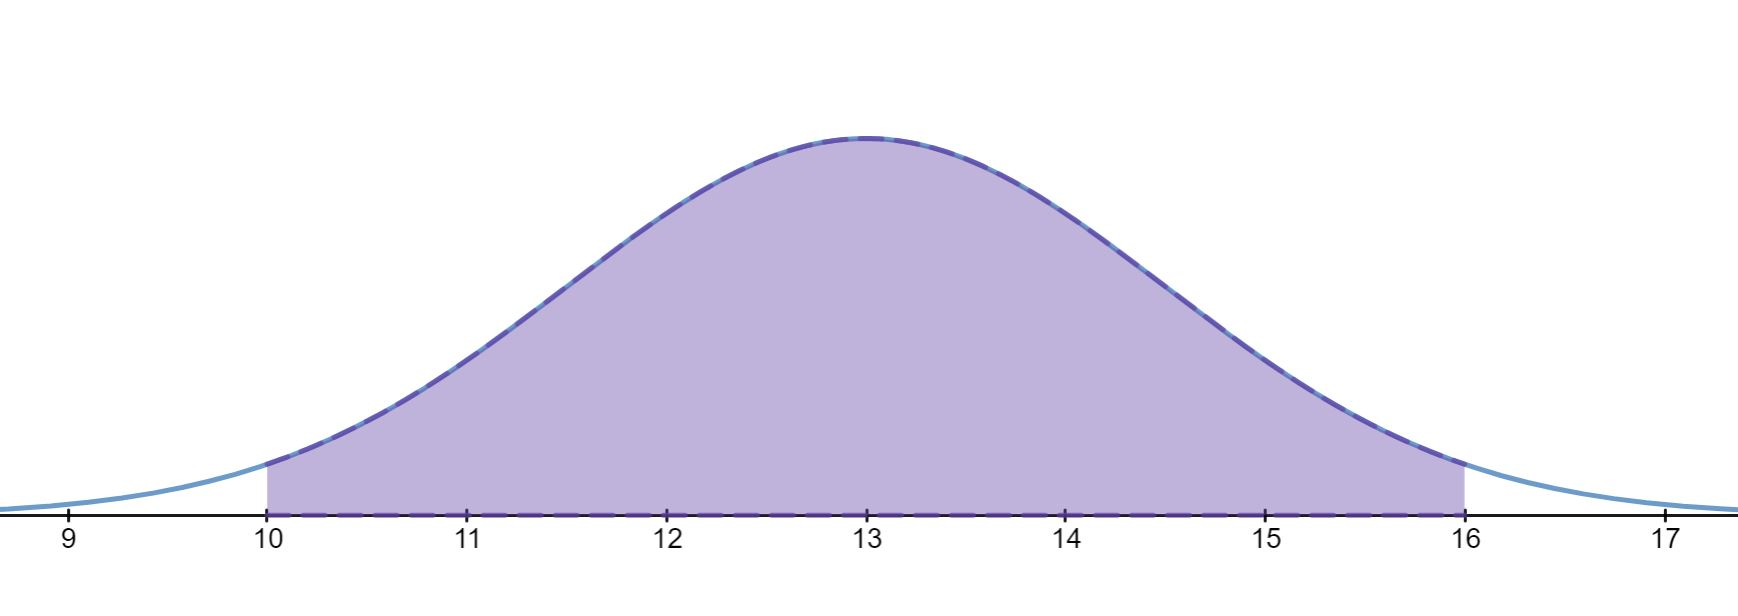
\includegraphics[height=1in]{140H5pic4.jpg}
 \end{image}
 $$\mbox{Area}=\answer{0.9544}$$
\end{problem}

\begin{problem}\label{prob:140hom5prob3}
Let $X\sim N(25, 2.2)$.  Use GoogleSheets to Find the shaded area.  State your answer to SIX decimal places.
\begin{image}
   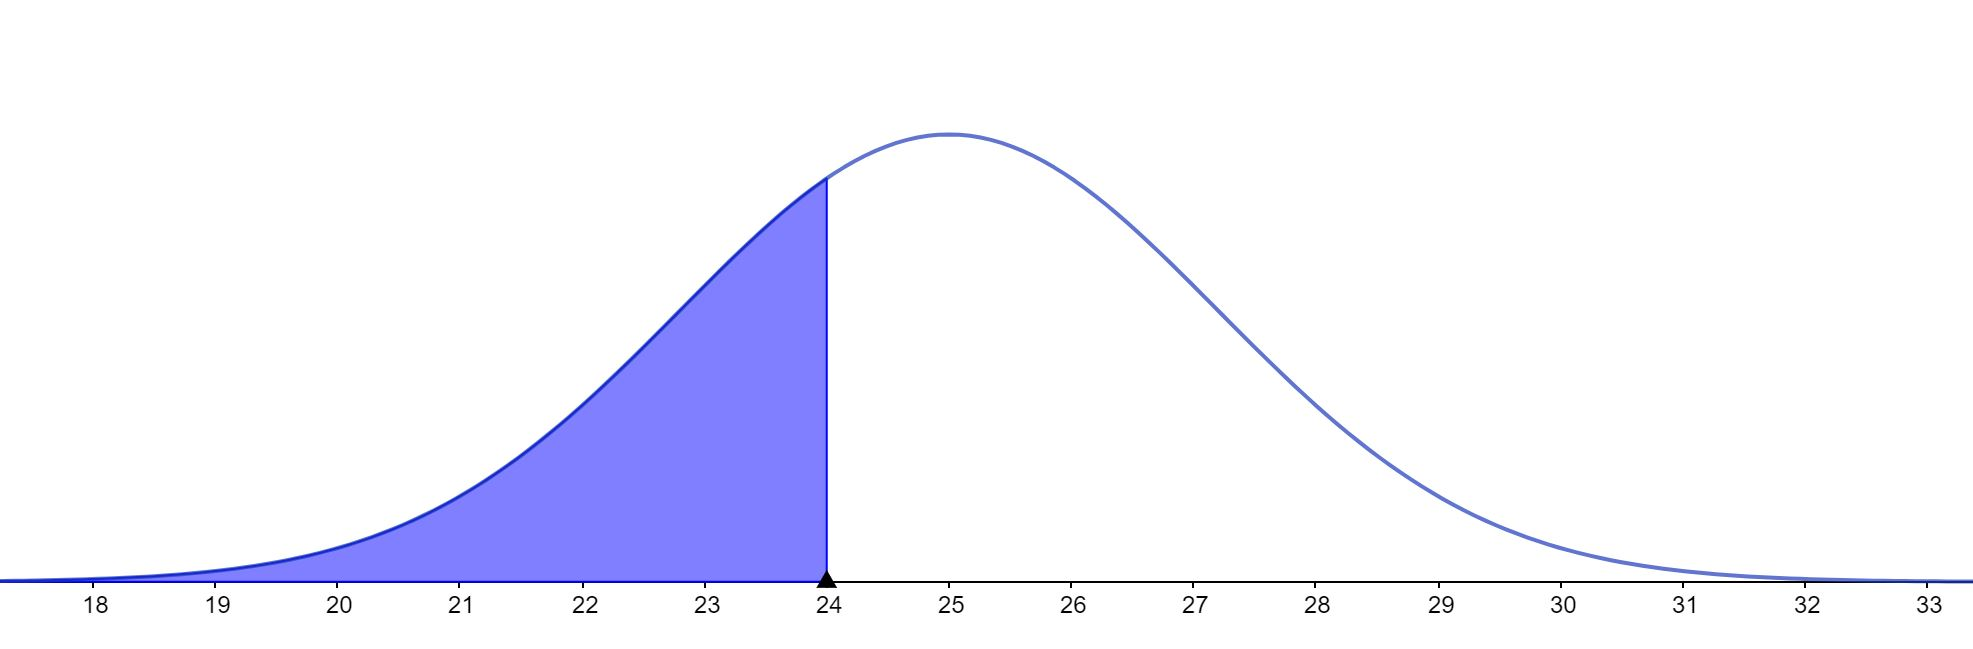
\includegraphics[height=1in]{140H5pic1.jpg}
 \end{image}
 $$\mbox{Area}=\answer{0.324718}$$
 \begin{image}
   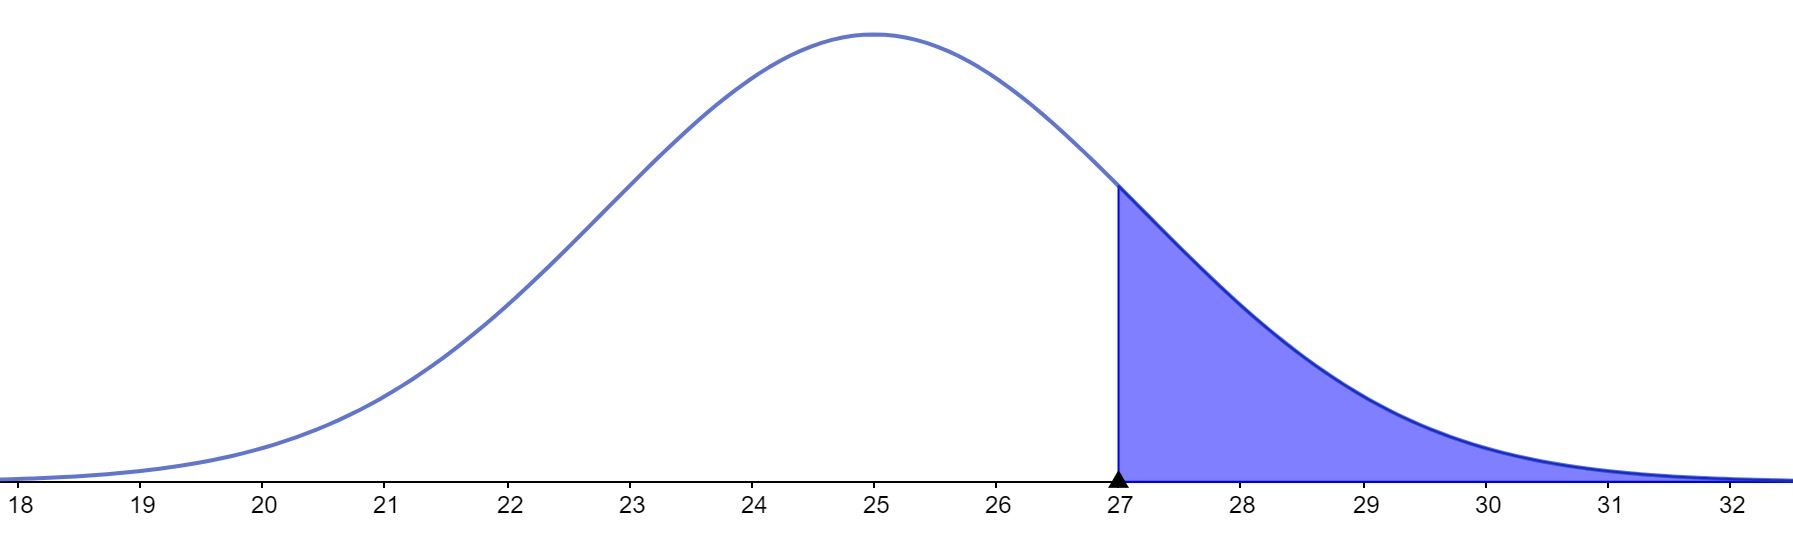
\includegraphics[height=1in]{140H5pic2.jpg}
 \end{image}
 $$\mbox{Area}=\answer{0.181651}$$
 \begin{image}
   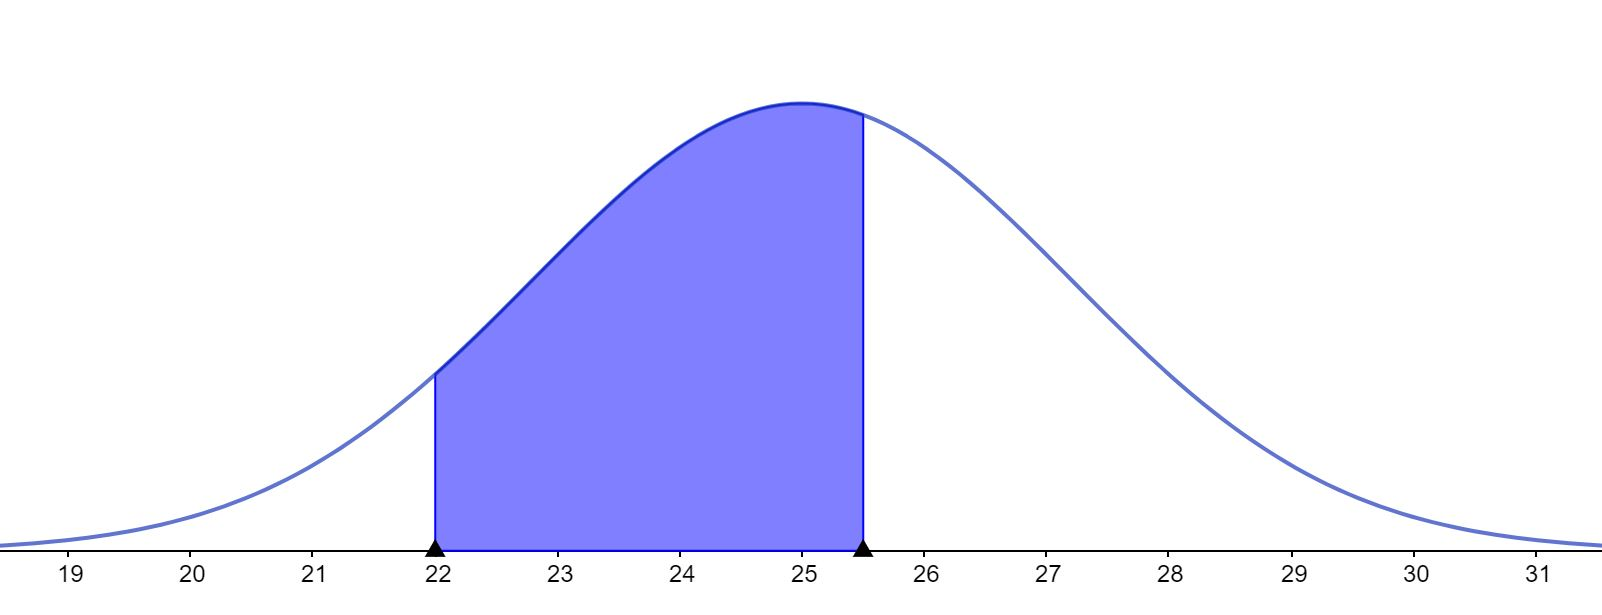
\includegraphics[height=1in]{140H5pic3.jpg}
 \end{image}
 $$\mbox{Area}=\answer{0.503553}$$
\end{problem}

\begin{problem}\label{prob:140hom5prob4} Let $X\sim N(32.6, 4.3)$.  Use GeoGebra to find the 70th percentile.  Geogebra gives answers to four decimal places.  State your answers using all of the digits from GeoGebra.
\begin{center}  
\geogebra{emwxhga2}{800}{600}  
\end{center}
$$70\mbox{th percentile}=\answer{34.8549}$$
\end{problem}
\end{document}